\section{Materialien}
\subsection{Hardware}
Zur Ausführung der MArC-Software sind diverse Hardware-Komponenten Voraussetzung. Diese Komponenten werden nachfolgend beschrieben und deren Kontext im System näher erläutert.
\subsubsection{Computer zur Ausführung der Unity-Simulation}
Die Anwendung, welche aus Unity\textsuperscript{\cite{website:Unity}} heraus erstellt wurde, benötigt einen Host-Computer, welcher sowohl mit dem HTC Vive Head-Mounted Display kompatibel, als auch leistungsstark genug sein muss, um das Rendering der Simulation mit ausreichend hoher Bildrate ausführen zu können.

\subsubsection{Computer zur Ausführung der Tracking-Anwendung}
\subsubsection{HTC Vive} \todo {Laura}
Bei der HTC Vive handelt es sich um ein Head-Mounted Display, welches von HTC in Kooperation mit Valve\textsuperscript{\cite{website:Valve}} produziert wird. Vorgestellt wurde dieses am 1. März 2015 im Vorfeld der Mobile World Congress\textsuperscript{\cite{website:mobileworldcongress}}.\\
Die Auflösung des Displays beträgt insgesamt $2160\times1200$ Pixel, was $1080x1200$ Pixeln pro Auge enstpricht. Die Brille bietet ein Sichtfeld von bis zu $110^\circ$ bei einer Bildwiederholrate von $90\,Hz$\textsuperscript{\cite{website:HTC_Vive}}. Zur Positionsbestimmung im Raum wird die Lighthousetechnologie von Valve genutzt. Zusätzlich sind neben einem Gyrosensor auch ein Beschleunigungsmesser und ein Laser-Positionsmesser verbaut. Mittels speziellen Game-Controllern wird eine Interaktion mit virtuellen Objekten ermöglicht. Die eingebaute Frontkamera wird für dieses Projekt nicht verwendet. Stattdessen wird auf die Ovrvision Pro zurückgegriffen, die im Folgenden in \ref{ovrvision} beschrieben wird.

\subsubsection{Spielfeldkamera} \todo {Vera}
IDS uEye 164xLE

\subsubsection{Leap Motion} \todo {Laura}	
Bei der Leap Motion\textsuperscript{\cite{website:LeapMotion}} handelt sich um ein $7,6\times3\times1,3\,cm$ großes Gerät, welches es mit Hilfe von Sensoren möglich macht, Hand- und Fingerbewegungen als Eingabemöglichkeit zu nutzen. Die Idee dahinter ist, eine Eingabegerät analog zu Maus zu schaffen, welches keinen direkten Kontakt bzw. keine Berührung benötigt. Hergestellt wird die Leap Motion von der Firma Leap Motion, Inc., die ihren Hauptsitz in Amerika hat. Gegründet wurde die Firma am 1. November 2010. \\
Wie auf Abbildung \ref{fig:leapMotion} erahnt werden kann, besteht das Gerät im wesentlich aus zwei integrierten weitwinkel Kameras und drei einfachen Infrarot LEDs. Die LEDs haben jeweils eine Wellenlänge von $850\,nm$. Der durch die beiden Kameras aufgespannte Interaktionsraum der Leap Motion ähnelt einer umgedrehten Pyramide, mit einem Flächeninhalt von knapp $243\,cm{^2}$. \\
Für das Projekt wurde die Orion beta software, die in \ref{OBS} näher beschrieben wird. Diese Software ermöglicht unter anderem eine Erweiterung der Reichweite der Leap Motion von $60\,cm$ auf $80\,cm$. Diese Reichweite ist durch die Ausbreitung der LED Lichter räumlich begrenzt. Die Lichtintensität der LEDs ist wiederum durch den maximalen Strom, der über die USB-Verbindung fließt beschränkt. \\

\subsection{Marker}\todo {Laura}
\subsubsection{ArUco Marker}\todo {Laura}
Da sowohl für die Marker, die für den eigentlichen Trackingalgorithmus verwendet werden, als auch für säntliche Marker, die zur Kalibrierung des Systems zum Einsatz kommen ArUco Marker verwendet werden, werden diese im Folgenden kurz erläutert.\\
ArUco Marker bestehen ähnlich wie QR-Codes aus einer zweidimensionalen Matrix, aus schwarzen und weißen Quadraten, die die kodierten Daten binär darstellen. Die ArUco Bibliothek kann für Augmented Reality Anwendungen genutzt werden und basiert ausschließlich auf der OpenCV Bibliothek. 
 
\subsubsection{Trackingmarker}\todo {Laura}
Das System umfasst zwölf Marker über die das Tracking realisiert wird. Alle Marker stimmen in Form und Farbe, sowie Material und Oberflächenbeschaffenheit überein. Sie sind würfelförmig und haben eine Kantenlänge von $46\,mm$. Die Kanten sind in einem Winkel von $45^\circ$ angefast. Die Marker bestehen aus Aluminium, welches glasperlgestrahlt ist um eine matte Oberfläche zu erzeugen. Auf die Oberseite des Markers ist mittig ein grünes Quadrat mit einer Kantenlänge von $40\,mm$ aufgebracht. Auf diesem ist, ebenfalls mittig, ein $35\,mm$ großer ARUCO-Marker, welcher aus dem $\texttt{DICT\_4X4\_50}$ generiert wurde und einen Rand von einem bit hat. Jeder Marker hat einen einzigartigen ARUCO-Marker, der einer Id von 1--12 entspricht.


	\begin{figure}[H]
		\center 
		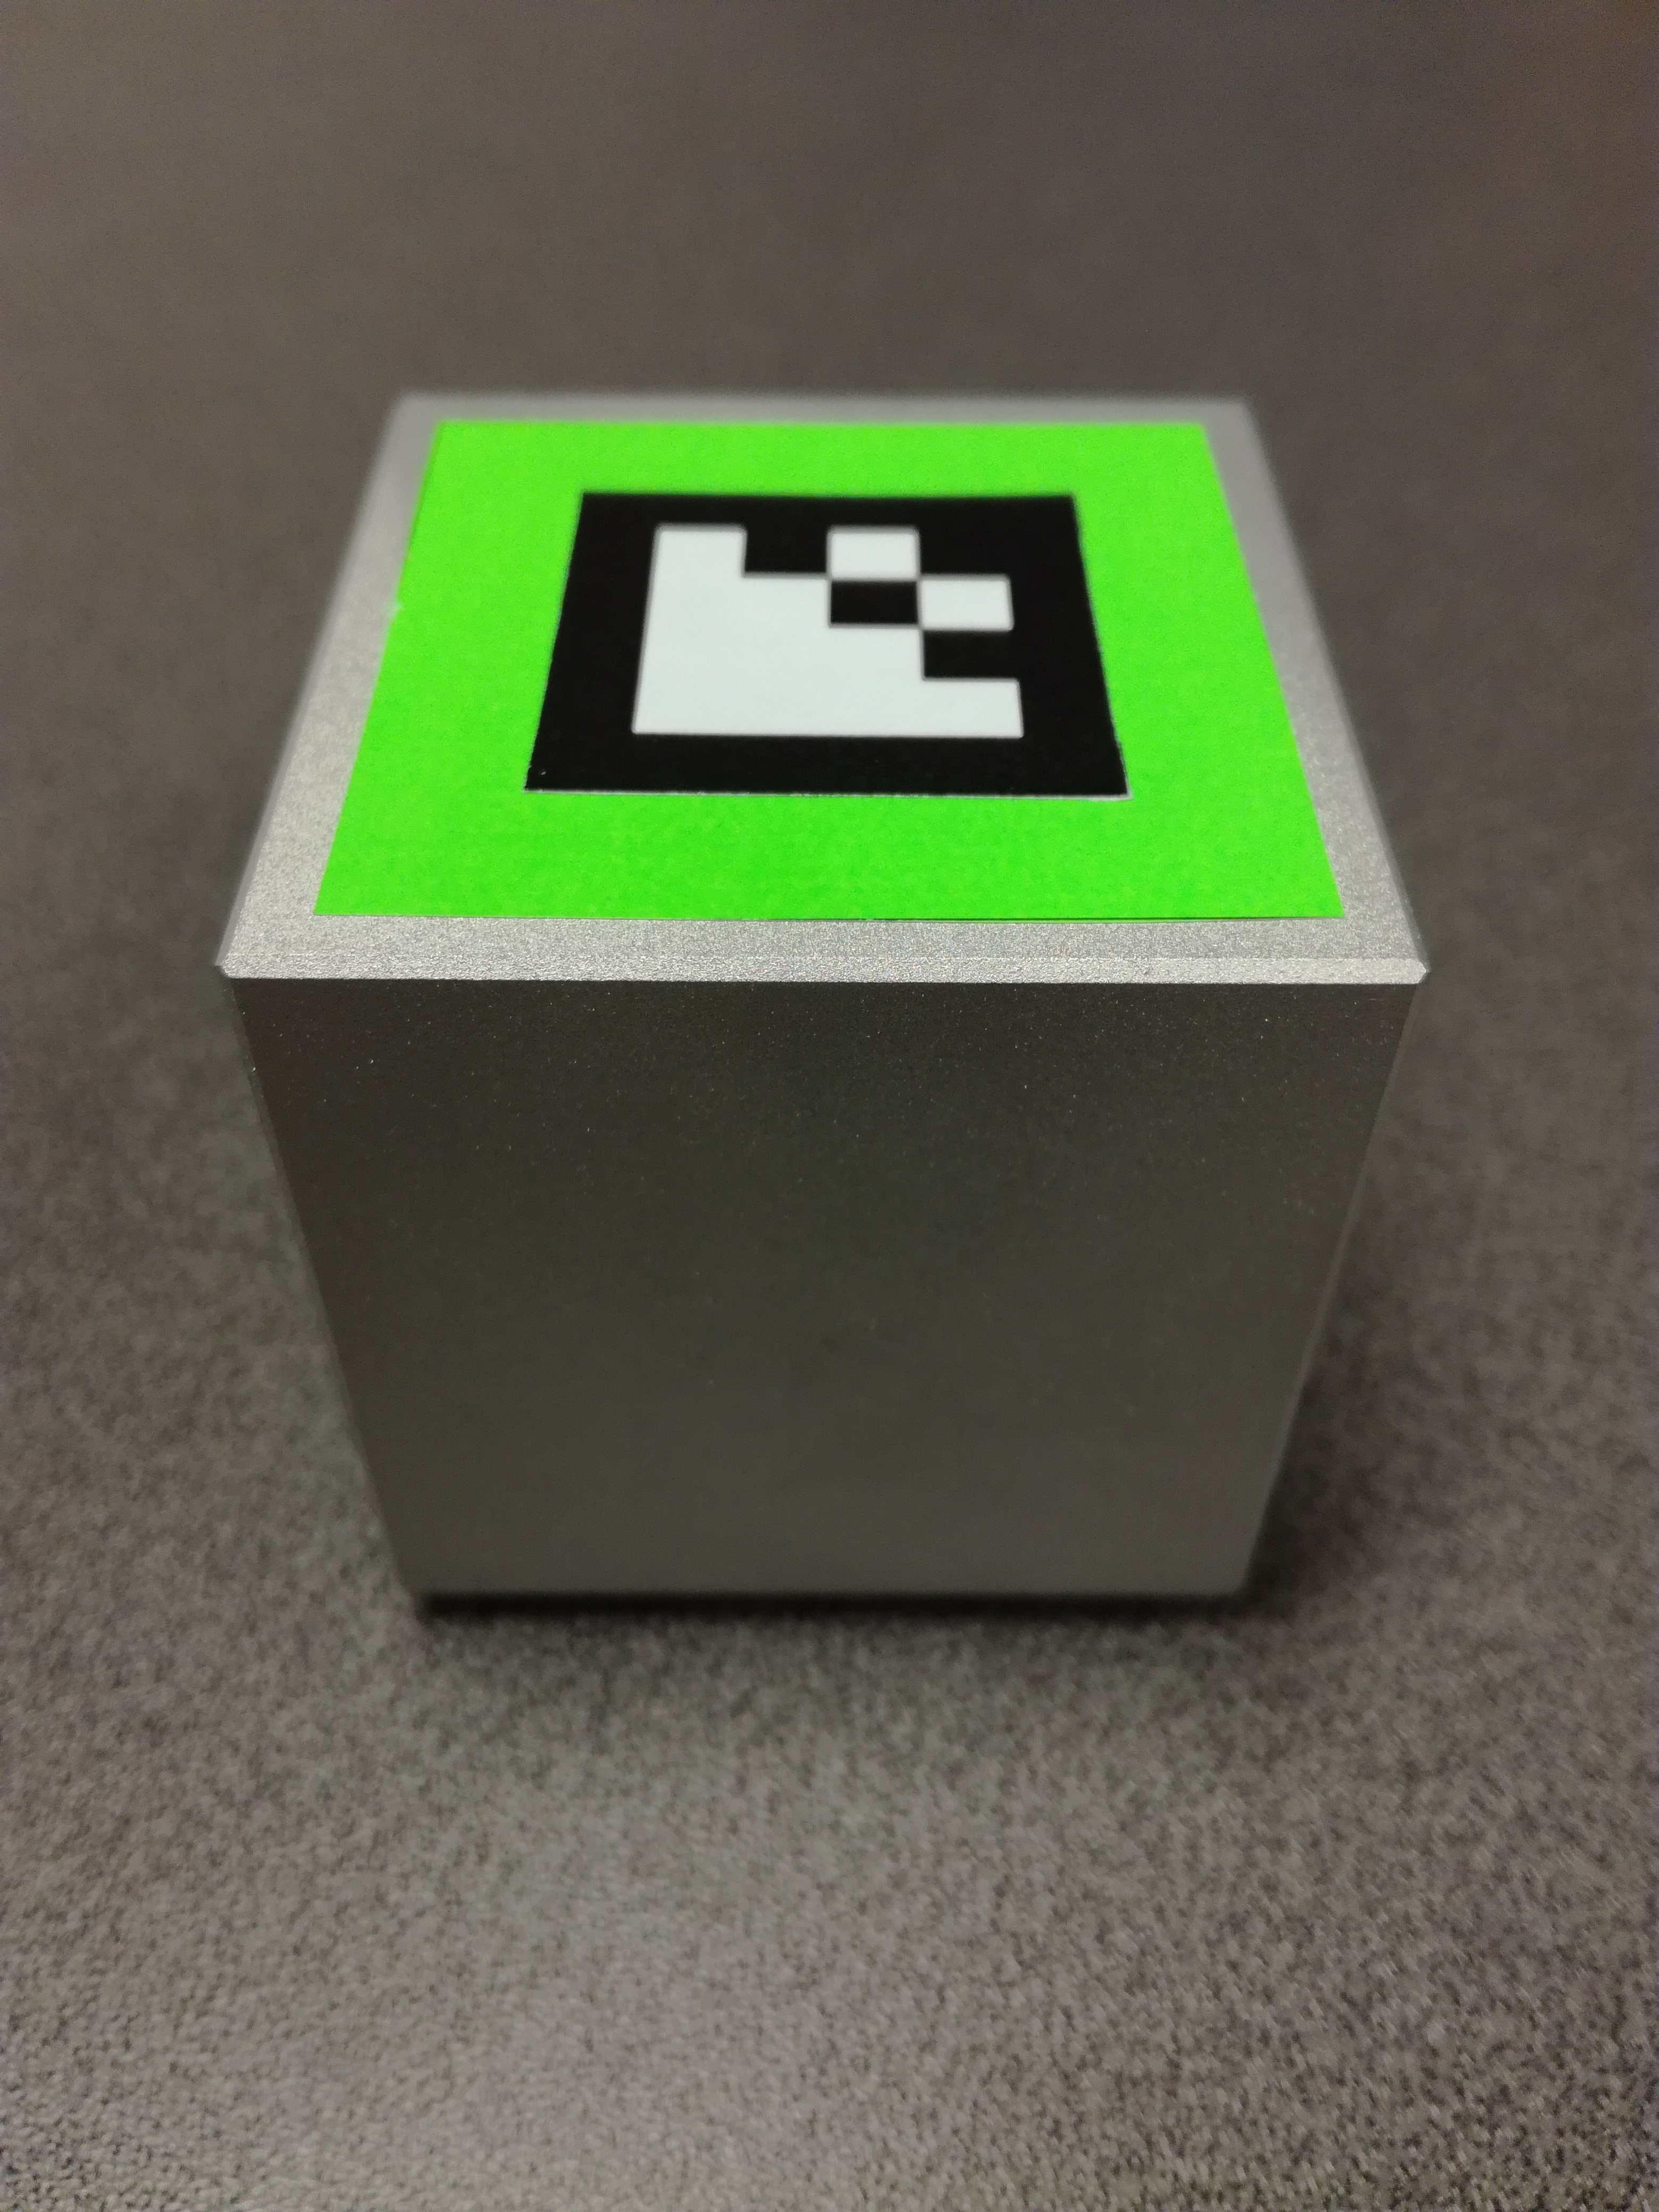
\includegraphics[trim = 0mm 280mm 0mm 150mm, clip, width=6cm]{Bilder/tracking-marker.jpg}
			\label{fig:marker}
			\caption{Trackingmarker mit der ID \textcolor{red}{??}.}
	\end{figure}
	
\subsection{Obsolete Hardware}\label{sec:obsoleteHardware}
Im Laufe eines Projekts nach Art von MArC ist es kaum vermeidbar, dass die gesetzten Projektziele reevaluiert werden müssen. Die Gründe hierfür können vielfältig sein. Beispielsweise könnte die Fertigstellung eines bestimmten Teils des Projekts deutlich länger gedauert haben als geplant, oder es könnte sich herausgestellt haben, dass bestimmte Komponenten zueinander nicht kompatibel sind.

Im vorliegenden Projekt trat eine Kombination der beiden oben genannten Gründe auf. Das Betreiben der Ovrvision Pro am US-Bus verschiedener während der Entwicklung verwendeter Rechner stellte sich als unberechenbar und damit leider unbenutzbar heraus. Die Kamera sorgte während der Ausführung von Unity dafür, dass mit allen anderen Geräten, die ebenfalls per USB angeschlossen waren, unterschiedlichste Probleme auftraten. Als die Situation nach dem Verbinden der Kamera in der teilweisen Zerstörung eines Mainboards gipfelte, wurde die Entscheidung getroffen, die Ovrvision nicht länger als Gerät in der Entwicklung zu verwenden.

Stattdessen war zu diesem Zeitpunkt die Idee, eine gewöhnliche Webcam zu verwenden, um die Realisierung von Augmented Reality dennoch zu ermöglichen, wenn auch ohne den Stereo-3D-Effekt, welchen die Ovrvision nativ bereitgestellt hätte.

Im weiteren Verlauf des Projekts führte eine lange Zeit ungeklärte, starke Abweichung der Positionen der realen und virtuellen Marker zur Neuordnung der Projektprioritäten. Dies hatte zur Folge, dass letztendlich auch die Webcam als Plattform für die Umsetzung der AR-Fähigkeiten von MArC aufgegeben wurde.

Nachfolgend werden die Eigenschaften und technischen Daten beider Geräte kurz beschrieben.
\subsubsection{Ovrvision Pro}\label{ovrvision}
Die Ovrvision Pro ist eine kompakte Stereokamera, welche über USB 3.0 mit dem Rechner verbunden werden kann\textsuperscript{\cite{website:ovrvision}}. Sie ist kompatibel mit Programmen wie Unity, welches für das Projekt benutzt wurde und in \ref{unity} beschrieben wird.

Die Bildmodi der Kamera sind in Tabelle~\ref{tab:ovrRes} aufgeführt.

\begin{table}
	\centering
	\begin{tabular}{|c|c|c|c|}
		\hline
		\Absatzbox{}
		\textbf{Örtliche Auflösung}& \textbf{Zeitliche} & \multicolumn{2}{c|}{\textbf{Bildwinkel}}\\
		\cline{3-4}
		\Absatzbox{}
		\textbf{pro Auge}& \textbf{Auflösung} & \textbf{Horizontal} & \textbf{Vertikal}\\
		\hline
		$2560\times1920$ & $15$\,fps & $115^\circ$ & $105^\circ$\\
		\hline
		$1920\times1080$ & $30$\,fps & $87^\circ$ & $60^\circ$\\
		\hline
		$1280\times960$ & $45$\,fps & $115^\circ$ & $105^\circ$\\
		\hline
		$1280\times800$ & $60$\,fps & $115^\circ$ & $90^\circ$\\
		\hline
		$960\times950$ & $60$\,fps & $100^\circ$ & $98^\circ$\\
		\hline
		$640\times480$ & $90$\,fps & $115^\circ$ & $105^\circ$\\
		\hline
		$320\times240$ & $120$\,fps & $115^\circ$ & $105^\circ$\\
		\hline
	\end{tabular}
	\caption{Bildmodi der Ovrvision Pro Stereokamera.\textsuperscript{\cite{website:ovrvisionProduct}}}
	\label{tab:ovrRes}
\end{table}

\begin{figure}[H]
	\centering
	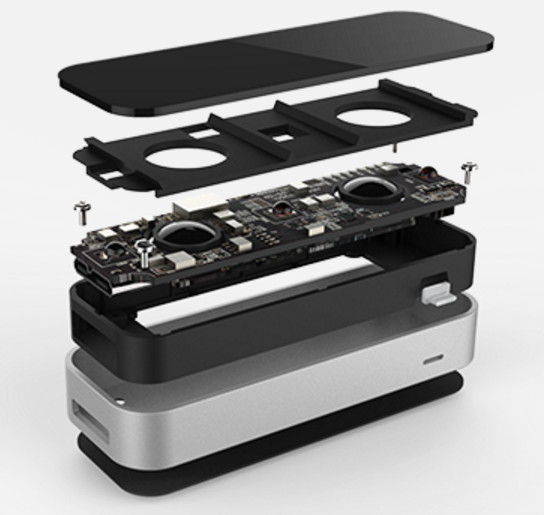
\includegraphics[width=6cm]{Bilder/leap-motion.png}			
		\caption{Explosionszeichnung der Leap Motion.\textsuperscript{\cite{website:LeapMotionBlog}}}
		\label{fig:leapMotion}
\end{figure}
	
\subsubsection{Webcam}

\subsection{Software}
\subsubsection{Unity}\label{unity}\todo[inline]{Paul oder Lukas}
Unity ist eine sogenannte Spiel-Engine, also eine Entwicklungs- und Laufzeitumgebung, die speziell auf die Entwicklung von 3D-Spielen ausgelegt ist. Die Software wurde am 6. Juni 2005 veröffentlicht\textsuperscript{\cite{haas2014history}} und wird von Unity Technologies\textsuperscript{\cite{website:Unity}} entwickelt und vertrieben. In der Spieleentwicklung ist Unity weit verbreitet, so werden beispielsweise $34\,\%$ der kostenfreien Top-1000-Spiele im mobilen Sektor mit Unity entwickelt\textsuperscript{\cite{website:UnityPR}}.

Unity bietet eine sehr breite Plattformunterstützung\textsuperscript{\cite{website:UnityMultiPlatform}} und erlaubt ebenso die Entwicklung für Head-Mounted-Displays, wie etwa die Oculus Rift\textsuperscript{\cite{website:UnityOculus}\cite{website:UnityVRoverview}} oder auch die in diesem Projekt verwendete HTC Vive.\textsuperscript{\cite{website:UnityVRoverview}}

Die zu Beginn des Projekts verwendete Stereo-Kamera Ovrvision Pro stellt ein Software-Development-Kit (SDK) für Unity (Version 5) zur Verfügung.\textsuperscript{\cite{website:ovrvisionSetup}} Da das endgültige Resultat des Projekts die Verwendung der Ovrvision Pro nicht mehr vorsieht, wie in~\ref{sec:obsoleteHardware} beschrieben, wird auf eine weitere Beschreibung dieses SDKs verzichtet.

\subsubsection{Visual Studio} \todo[inline] {Laura}
\subsubsection{OpenCV} \todo[inline] {Vera}
Wo führen wir die dlls auf die du erzeugt hast??

% Wie in "`Unity"' oben beschrieben, denke ich, dass wir uns das folgende sparen können, oder?
%\subsubsection{Ovrvision Pro SDK} \todo[inline] {Paul oder Lukas}

\subsubsection{Leap Motion SDK} \todo[inline] {Laura}
\textcolor{red}{
Once the image data is streamed to your computer, it’s time for some heavy mathematical lifting. Despite popular misconceptions, the Leap Motion Controller doesn’t generate a depth map – instead it applies advanced algorithms to the raw sensor data.}

The Leap Motion Service is the software on your computer that processes the images. After compensating for background objects (such as heads) and ambient environmental lighting, the images are analyzed to reconstruct a 3D representation of what the device sees.

Next, the tracking layer matches the data to extract tracking information such as fingers and tools. Our tracking algorithms interpret the 3D data and infer the positions of occluded objects. Filtering techniques are applied to ensure smooth temporal coherence of the data. The Leap Motion Service then feeds the results – expressed as a series of frames, or snapshots, containing all of the tracking data – into a transport protocol.

Through this protocol, the service communicates with the Leap Motion Control Panel, as well as native and web client libraries, through a local socket connection (TCP for native, WebSocket for web). The client library organizes the data into an object-oriented API structure, manages frame history, and provides helper functions and classes.

From there, the application logic ties into the Leap Motion input, allowing a motion-controlled interactive experience. Next week, we’ll take a closer look at our SDK and getting started with our API.\textsuperscript{\cite{website:LeapMotionBlog}}

\subsubsection{Orion Beta Software} \label{OBS}

\subsubsection{uEye SDK}\todo[inline] {Vera}
\subsubsection{Steam VR}\todo[inline] {Paul oder Lukas}


\newpage